\documentclass[10pt]{article}
\usepackage[T1]{fontenc}
\usepackage[utf8]{inputenc}
\usepackage[english]{babel}
\usepackage{lmodern}
\usepackage{amsmath,amssymb,array,longtable,geometry,microtype}
\usepackage{tikz}
\geometry{paperwidth=6.5in,paperheight=9in,margin=0.62in}
\pagestyle{empty}
\setlength{\parindent}{1em}
\setlength{\parskip}{0.18em}
\setlength{\abovedisplayskip}{0.45em}
\setlength{\belowdisplayskip}{0.45em}
\emergencystretch=2em
\hbadness=10000
\hfuzz=2pt
\newcommand{\TeubnerMark}{\begin{center}\setlength{\fboxsep}{1pt}\fbox{\scriptsize\bfseries B\,G\,T}\end{center}}
\begin{document}
\small

\begin{center}
{\large Dr. Paul Gordan's Lectures}\\[0.45em]
{\scriptsize ON}\\[0.65em]
{\LARGE\bfseries INVARIANT THEORY.}\\[1.6em]
{\scriptsize EDITED}\\[0.45em]
{\scriptsize BY}\\[0.65em]
{\bfseries Dr. Georg Kerschensteiner.}\\[1.6em]
{\scriptsize FIRST VOLUME:}\\[0.45em]
{\large\bfseries DETERMINANTS.}\\[1.5em]
\TeubnerMark
\vfill
{\small LEIPZIG,}\\[0.25em]
{\scriptsize PRINTED AND PUBLISHED BY B. G. TEUBNER.}\\[0.25em]
{\small 1885.}
\end{center}

\newpage

\begin{center}
{\small TO}\\[0.9em]
{\Large\bfseries CHARLES HERMITE}\\[0.8em]
{\scriptsize DEDICATES}\\[0.8em]
{\small AS A TOKEN OF HIS VENERATION}\\[0.8em]
{\scriptsize THIS LECTURE}\\[0.8em]
{\bfseries PAUL GORDAN.}
\end{center}

\newpage

\begin{center}
{\bfseries Preface.}
\end{center}

A few years ago German mathematical literature was enriched by an adaptation of Faà di Bruno's “Introduction to the Theory of Binary Forms,” so that we are now in possession of three works -- Salmon, Clebsch, and Faà di Bruno -- whose contents extend over the modern theory of invariants and covariants. The present work stands in close connection with Clebsch; indeed it has arisen from those ideas which Gordan had already deposited in that book when it appeared. But what at that time appeared as a co-ordinate question has now become the chief aim of this work: I mean the fundamental investigations concerning the finiteness of the system of forms and the closely connected questions concerning the relations among the individual forms. This has become the fundamental standpoint of these lectures, around which all other invariant-theoretical questions are grouped and from which they are to receive their illumination and meaning here. It has proved fruitful in every direction. Through it, however, the limits were also determined within which the present work was to become a theory of invariants, that is, within which the discipline, now already diversely articulated, was to receive an exhaustive treatment.

It is therefore natural that, in adhering unswervingly to precisely this aim, Gordan used in all his investigations the symbolism founded by Aronhold, and that these lectures thus also attach themselves in form to the excellent work of Clebsch. Since the death of that master, however, invariant theory has become wholly independent. Whereas, after arising from number theory, it first attached itself to the analytic geometry of the plane, its significance has today grown essentially. It has become an end in itself, and may therefore today be regarded as that discipline which brings the purely formal laws of algebra to expression. This should be kept in mind when, in the present work, the laws of invariant theory are applied chiefly only to questions from the theory of algebraic equations, insofar as, as in the third volume, the theory of ternary forms does not here and there give rise to geometric interpretations, or the theory of prime forms does not connect these laws with the theory of differential equations. Its connection with problems of the calculus of variations and certain problems of physics could of course be touched on all the less, since even all the essential services which it has rendered to geometry receive no discussion in these lectures.

Insofar, however, as the lectures move within the limits thus marked out, they will not only be an introduction to the theory of invariants, but will guide the reader up to the present standpoint to which this discipline has been advanced by the eminent work of Hermite and Brioschi, Cayley, Sylvester and Salmon, Aronhold, Clebsch and Gordan.

Of those questions which could not be considered here, the more important ones have been taken up in Salmon's “Lectures on the Algebra of Linear Transformations,” so that the two sets of lectures together provide a complete picture of the stage of development at which invariant theory presently stands.

The first part of this work, which is concerned with the theory of determinants, may be regarded as preparation for the other two parts. The symbolic methods make the need for a preliminary theory of determinants unavoidable, and, on the other hand, it is precisely determinant relations that repeatedly give occasion for relations among forms.

This aim of the first part, to make familiar the means that must be presupposed in the theory of invariants, imposed on it a certain limitation of material; in compensation, however, computation with matrices receives a much fuller treatment than in other works on determinants. In its disposition this first part stands in close connection with Baltzer's long-recognized work of the same name. The latter, however, goes further in many investigations, as the aim of Baltzer's work, which sets itself more general problems, requires.

Here, in the theoretical part, only determinants in general are treated and their properties developed completely; special determinants, however, such as symmetric and continued-fraction determinants, receive no detailed discussion. The theory concludes with the consideration of corresponding matrices, which play a noteworthy role in several very recent invariant-theoretical works.

Naturally, with regard to the aim of this part, firm limits were also set for the application of the theory. Only the theory of linear equations, the properties of functional determinants, and the resultants receive detailed treatment, because of their outstanding importance for invariant theory. I had to refrain in general from the originally planned source citations; there is also no longer any great need for them, since for determinants these sources are indicated in detail in Baltzer's and Günther's relevant works, and for invariants in Salmon's textbooks and in the German adaptation of Faà di Bruno.

I should like to close these introductory remarks by expressing my warmest thanks to Professor Gordan for asking me to publish his lectures. I have subjected myself to a free and independent adaptation of them with all restraint of my own self, and I am satisfied if I have succeeded in bringing the ideas which govern his lectures to clear expression, whether through the arrangement and the developments themselves, or through the numerous examples and applications that I have woven into them according to my needs.

\begin{flushleft}
Nuremberg, July 1885.
\end{flushleft}
\begin{flushright}
Georg Kerschensteiner.
\end{flushright}

% --- Source pages 0010--0028; printed table of contents VIII--XI, blank XII, printed pages 1--14. ---

\begin{center}
{\bfseries Contents.}\\[0.35em]
{\bfseries First Part.}\\[0.35em]
{\bfseries Theory of Determinants.}
\end{center}

\begingroup\scriptsize\setlength{\tabcolsep}{2pt}
\begin{longtable}{>{\raggedleft\arraybackslash}p{0.55in}p{4.05in}>{\raggedleft\arraybackslash}p{0.35in}}
{\scriptsize Paragraph.} & & {\scriptsize Page}\\
\multicolumn{3}{>{\centering\arraybackslash}p{5.0in}}{\bfseries \S\,1. Permutation and Substitution.}\\
1. & Permutation & 1\\
2. & Derangement & 1\\
3. & Counting derangements by division & 2\\
4. & Concept of substitution & 3\\
5. & Kinds of substitutions & 5\\
6--9. & Construction of the different substitutions from one another & 7\\
10--12. & Classification of the different substitutions & 11\\[0.25em]
\multicolumn{3}{>{\centering\arraybackslash}p{5.0in}}{\bfseries \S\,2. Concept of determinants.}\\
13. & Use of substitutions for producing all terms of a determinant & 15\\
14. & Definition of the determinant & 17\\
15. & Calculation of the value of a determinant from its matrix & 19\\
16. & Method for setting up theorems on determinants & 21\\
17. & Transposition & 21\\
18. & Notations for a determinant & 23\\
19--20. & Interchange of columns and rows & 24\\
21--23. & Examples of interchanging columns and rows & 28\\[0.25em]
\multicolumn{3}{>{\centering\arraybackslash}p{5.0in}}{\bfseries \S\,3. First-order subdeterminants.}\\
24. & Concept of the first-order subdeterminant \(A_{ik}\) & 31\\
25--26. & Calculation of the subdeterminant \(A_{ik}\) & 32\\
27. & Examples & 33\\
28--29. & Expansion of the determinant by subdeterminants & 34\\
30. & Examples & 35\\
31--33. & Relations between first-order minors \(A_{ik}\) & 36\\
34. & Applications of these relations & 38\\
35--36. & Addition of determinants & 40\\
37. & Examples & 40\\
38. & Multiplication of a determinant by a factor \(\lambda\) & 42\\
39. & Combination of the addition and multiplication laws & 42\\
40. & Applications of the theorems of this section & 43\\[0.25em]
\multicolumn{3}{>{\centering\arraybackslash}p{5.0in}}{\bfseries \S\,4. Partial determinants of higher order.}\\
41. & Concept of the second-order subdeterminant & 47\\
42. & Relation of the second-order minor to the first-order minor & 48\\
43. & Example & 49\\
44--45. & Concept of the minor of \(p^{\mathrm{th}}\) order & 50\\
46--48. & Calculation of the minor of \(p^{\mathrm{th}}\) order & 51\\
49--51. & Corresponding determinant of the minor of \(p^{\mathrm{th}}\) order & 53\\
52. & Examples & 57\\[0.25em]
\multicolumn{3}{>{\centering\arraybackslash}p{5.0in}}{\bfseries \S\,5. Expansion of the determinant into a sum of products of corresponding determinants.}\\
\multicolumn{3}{>{\centering\arraybackslash}p{5.0in}}{(Laplace's theorem.)}\\
53. & Expansion into a sum of products from minors of order \((n-2)\) and their corresponding subdeterminants & 59\\
54. & Expansion into a sum of products from minors of order \((n-3)\) and their corresponding minors & 61\\
55. & General case & 61\\
56--58. & Applications of Laplace's theorem to forming relations between minors & 62\\
59--61. & Calculation of determinants with the help of Laplace's theorem & 65\\
62. & Expansion of the determinant by products of elements of two intersecting rows or columns & 67\\
63--66. & Expansion of the determinant by products of elements of two pairs of intersecting rows or columns & 68\\
67. & Concept of bordering & 72\\[0.25em]
\multicolumn{3}{>{\centering\arraybackslash}p{5.0in}}{\bfseries \S\,6. Multiplication of determinants.}\\
68--71. & First way to multiply determinants & 73\\
72. & Second way of multiplication & 77\\
73. & Symmetric determinants & 77\\
74. & Linear relations between minors of symmetric determinants & 78\\
75--84. & Multiplication of matrices which do not represent determinants & 79\\[0.25em]
\multicolumn{3}{>{\centering\arraybackslash}p{5.0in}}{\bfseries \S\,7. Adjoint determinants and corresponding matrices.}\\
85. & Definition of the adjoint determinant & 88\\
86. & Value of the adjoint determinant & 89\\
87--88. & Value of a minor of the adjoint determinant & 89\\
89. & Example & 93\\
90. & Definition of the corresponding matrices & 94\\
91--94. & Theorem on corresponding matrices & 95\\
95. & Example & 99\\[0.35em]
\multicolumn{3}{>{\centering\arraybackslash}p{5.0in}}{\bfseries Second Part.}\\
\multicolumn{3}{>{\centering\arraybackslash}p{5.0in}}{\bfseries Applications of determinant theory.}\\
\multicolumn{3}{>{\centering\arraybackslash}p{5.0in}}{\bfseries \S\,8. Systems of linear equations and their solution.}\\
96--97. & Solution of a system (I) of \(n\) linear homogeneous equations with \(n\) unknowns & 101\\
98. & Concept of the resultant of homogeneous linear equations & 102\\
99--101. & Solution of system (I), when its resultant together with all minors of order \((\mu-1)\) vanish & 103\\
102. & Solution of \(n-1\) homogeneous equations with \(n\) unknowns & 106\\
103. & Uniqueness of this solution & 107\\
104. & Examples & 108\\
105--110. & Solution of \(\mu\) homogeneous equations with \(n\) unknowns, when \(n>\mu+1\) (with a second proof of the theorem on corresponding matrices) & 109\\
111. & Solution of a system of \(n\) non-homogeneous equations with \(n\) unknowns & 117\\
112. & Discussion of the solution & 118\\
113. & Examples & 118\\[0.25em]
\multicolumn{3}{>{\centering\arraybackslash}p{5.0in}}{\bfseries \S\,9. Functional determinants.}\\
114. & Definition of the functional determinant & 120\\
115. & The functional determinant is an alternating function & 121\\
116. & Representation of a minor of the functional determinant & 121\\
117--118. & Product theorem for functional determinants & 122\\
119. & The functional determinant as a product of partial differential quotients & 125\\
120. & Differential quotients of minors of the functional determinant & 127\\
121--125. & Functional determinant of a system of functions between which a relation exists & 128\\[0.25em]
\multicolumn{3}{>{\centering\arraybackslash}p{5.0in}}{\bfseries \S\,10. The greatest common factor.}\\
126--127. & Euclidean procedure for two integers \(a\) and \(b\) & 131\\
128. & Greatest common divisor of \(f(x)\) and \(\varphi(x)\) & 133\\
129. & Exposition of the problems to be solved in this section & 135\\
130--131. & Definition and calculation of the resultant \(R_{f,\varphi}\) of \(f\) and \(\varphi\) & 136\\
132--136. & Calculation of a common factor of degree \((\varrho+1)\) of \(f\) and \(\varphi\) & 139\\
137. & Example & 143\\[0.25em]
\multicolumn{3}{>{\centering\arraybackslash}p{5.0in}}{\bfseries \S\,11. Properties of the resultant \(R_{f,\varphi}\) of two functions \(f(x)\) and \(\varphi(x)\).}\\
138. & Presentation of the method for determining these properties & 145\\
139. & Proof: \(R_{f,\varphi}=(-1)^{n\cdot m}R_{\varphi,f}\) & 146\\
140. & Proof: \(R_{f,\varphi}=R_{x^n\varphi(1/x),\,x^mf(1/x)}\) & 146\\
141. & Proof: \(R_{f(\lambda x),\,\varphi(\lambda x)}=\lambda^{m\cdot n}R_{f,\varphi}\) & 147\\
142. & Intersection points of two curves of orders \(m\) and \(n\) & 148\\
143--144. & The resultant as a functional determinant & 148\\
145. & Proof: \(R_{f+\varphi\cdot\psi,\,\varphi}=R_{f,\varphi}\), when \(\psi\) has degree \(q\) in \(x\), and \(q+n\leq m\) & 150\\
146. & Example: \(R_{f+\lambda\varphi,\,\varphi}=R_{f,\varphi}\) & 149\\
147. & Proof: \(R_{f(x+u),\,\varphi(x+u)}=R_{f,\varphi}\) & 152\\
148--150. & Reduction of Sylvester's form of \(R_{f,\varphi}\) to Bézout's form & 153\\
151. & Cayley's method for this reduction & 158\\
152. & Example & 161\\
153--154. & Proof: \(R_{f,\varphi\cdot\psi}=R_{f,\varphi}\cdot R_{f,\psi}\), when \(q+n\leq m\) & 162\\
155. & Examples & 164\\[0.25em]
\multicolumn{3}{>{\centering\arraybackslash}p{5.0in}}{\bfseries \S\,12. Fundamental theorem of algebra.}\\
156. & Transcendental part of the proof & 166\\
157. & Course of thought for the algebraic part of the proof & 167\\
158. & Classification of equations by the degree of their solvability & 167\\
159--160. & Every equation has a linear factor if it has any factor at all & 168\\
161--162. & Every equation must have a factor & 170\\[0.25em]
\multicolumn{3}{>{\centering\arraybackslash}p{5.0in}}{\bfseries \S\,13. Connection of the resultant with the roots of equations.}\\
163--164. & Calculation of the common root of two equations & 174\\
165--166. & Connection between coefficients and roots of an equation & 176\\
167. & Power sums of the roots & 178\\
168--172. & The resultant \(R_{f,\varphi}\) as product of differences of roots & 179\\[0.25em]
\multicolumn{3}{>{\centering\arraybackslash}p{5.0in}}{\bfseries \S\,14. The discriminant.}\\
173. & Definition of the discriminant & 185\\
174--177. & Its calculation & 186\\
178. & On the occurrence of a multiple root of \(f\) in the first derivative of \(f\) & 190\\
179--180. & Calculation of the double root of an equation \(f=0\) & 191\\
181. & Third proof that \(R_{f_1,f}=R_{f_1,f_2}\) & 193\\
182--183. & Examples & 194\\[0.25em]
\multicolumn{3}{>{\centering\arraybackslash}p{5.0in}}{\bfseries \S\,15. Simultaneous system of homogeneous linear Diophantine equations.}\\
\multicolumn{3}{>{\centering\arraybackslash}p{5.0in}}{(Appendix to \(\S\,8\).)}\\
184. & Finding integral solutions of one equation & 196\\
185. & Example & 198\\
186. & Solution of several simultaneous Diophantine equations & 198\\
187--189. & Integral positive solutions & 199
\end{longtable}
\endgroup

\newpage

\begin{center}
{\bfseries First Part.}\\[0.35em]
{\bfseries Theory of Determinants.}\\[0.6em]
{\bfseries \S\,1. Permutation and Substitution.}
\end{center}

1. \emph{Permutation.} If in a group of \(n\) elements -- we shall denote them by \(a,b,c\ldots h\) -- all possible interchanges of these elements are performed, then a series of new groups or complexes arises, differing only by the order of their elements, and these are commonly called permutations. The number of these permutations is
\[
N=n(n-1)\ldots3\cdot2\cdot1=n!,
\]
as is readily seen by observing that every permutation of \(n\) elements is obtained by combining each of the \(n\) elements with all permutations of the remaining \((n-1)\) elements. It is then also seen that among these \(N\) permutations \((n-1)!\) begin with \(a\), the same number with \(b,c\), and so on; and we agree to count every permutation that begins with the same element in the same class, so that all the permutations are thereby divided into \(n\) classes.

2. \emph{Derangement.} Instead of denoting the elements of a permutation by \(a,b,c\ldots h\), one prefers to introduce the expressions \(a_1,a_2,a_3\ldots a_n\), or still more simply the numbers \(1,2,3\ldots n\) appended to the letter \(a\), which are called indices or suffixes. We then call a permutation in which no higher index stands to the left before a lower one well ordered. If, on the other hand, a higher index lies to the left before a lower one, then the permutation is said to contain an inversion or derangement, and the number of these derangements is as large as the number which indicates how often lower indices occur to the right of a higher index. Thus, for example, the permutations
\[
(pqrs),\qquad (1\ 2\ 3\ 4\ 5)
\]
are well ordered; on the other hand the permutation
\[
(7\ 4\ 1\ 2\ 3\ 6\ 5)\quad\text{contains derangements: }6+3+1=10,
\]
namely 6 arising from the index 7, 3 as a consequence of the position of 4, and 1 as a consequence of the position of the index 6. Similarly the permutation \((3\ 5\ 4\ 1\ 2)\) contains the derangements \(31,32,54,51,52,41\), and \(42\), hence 7 in all.

3. \emph{Counting the derangements in a permutation by division.} To determine rapidly the number of derangements in a permutation, one can sometimes use the following method with advantage, especially when the permutation contains many elements.

We divide the permutation into 2 arbitrary parts:
\[
\begin{array}{r@{\ }l}
\text{the first group contains, in order, the indices} & i_1\,i_2\ldots i_\mu,\\
\text{the second group contains, in order, the indices} & k_1\,k_2\ldots k_\nu
\end{array}
\quad\Big\}\quad \nu+\mu=n.
\]
The total number of derangements is then formed

1) from those which arise from the group of the \(i\)'s alone,

2) from those which arise from the group of the \(k\)'s alone,

3) from those which the elements \(i\) form with respect to the \(k\)'s.

For the number of derangements of the third kind a simple formula can now be given; if one adds to this the number of inversions of the first and second kinds, which, since the groups in question contain fewer elements, can be found more easily than those of the whole permutation, then one obtains the total number. This summation formula is supplied by the theorem:
\begin{quote}
``The number of derangements of the third kind is equal to the sum of all indices of the group of the \(i\)'s minus the sum of the natural numbers from 1 to \(\mu\), where \(\mu\) denotes the number of elements of the first group.''
\end{quote}

\emph{Proof.} The number of these derangements of the third kind does not change if I first put the group of the \(i\)'s and the group of the \(k\)'s in good order among themselves. Let the first group then be \((J_1\,J_2\ldots J_\mu)\), the second \((K_1\,K_2\ldots K_\nu)\), so that the permutation is
\[
(J_1\ J_2\ldots J_\mu\mid K_1\ K_2\ldots K_\nu)\qquad(\nu+\mu=n).
\]
This new permutation has no derangements in the \(J_\varrho\) and none in the \(K_\varrho\); it still has, however, all derangements of the third kind. Their number splits into those coming from \(J_1\), those from \(J_2\), and so on, up to those from \(J_\mu\). The first part is evidently \(J_1-1\), since \(J_1\) forms inversions with \emph{all} smaller indices; the second part is \(J_2-2\), since \(J_2\) forms inversions with all smaller indices except the preceding \(J_1\); similarly, finally, the \(\mu^{\mathrm{th}}\) part is \(J_\mu-\mu\). Thus the total number is
\[
\begin{aligned}
Z&=J_1+J_2+J_3\ldots+J_\mu-(1+2+\cdots+\mu)\\
&=i_1+i_2+i_3\ldots+i_\mu-\frac{\mu(\mu+1)}{2}.
\end{aligned}
\]

Examples: \(\alpha)\) Given the permutation
\[
(3\ 7\ 9\ 8\ 1\ 5\ 2\ 6\ 4).
\]
We divide it arbitrarily by a vertical stroke into two groups:
\[
(3\ 7\ 9\ 8\mid1\ 5\ 2\ 6\ 4)=(i_1\ i_2\ i_3\ i_4\mid k_1\ k_2\ k_3\ k_4\ k_5)
\]
and put each of them in good order:
\[
(3\ 7\ 8\ 9\mid1\ 2\ 4\ 5\ 6)=(J_1\ J_2\ J_3\ J_4\mid K_1\ K_2\ K_3\ K_4\ K_5).
\]
Now
\[
i_1+i_2+i_3+i_4=3+7+8+9=27,\qquad
\frac{\mu(\mu+1)}{2}=\frac{4\cdot5}{2}=10,
\]
therefore the number of inversions is \(Z=27-10=17\), as is also found by direct counting. Adding to this the one inversion in the group of the \(i\)'s and the three in the group of the \(k\)'s, the total number is \(21\).

\(\beta)\) Given the permutation
\[
(7\ 3\ 6\ 2\ 4\ 1\ 5);
\]
we divide it into two parts:
\[
(7\ 3\ 6\mid2\ 4\ 1\ 5),
\]
then the sum is \(7+3+6=16\), the number of elements \(=3\). Thus the number of derangements of the third kind is
\[
16-\frac{3\cdot4}{2}=10.
\]
Indeed, if we put it in good order, we obtain
\[
(3\ 6\ 7\mid1\ 2\ 4\ 5),
\]
hence 2 derangements arising from 3, 4 arising from 6, and \(7-3=4\) arising from 7, in all 10. Adding the derangements of the \(i\)'s, \(=2\), and of the \(k\)'s, \(=2\), gives the total sum 14.

4. \emph{Concept of substitution.} The transfer from one permutation into another is effected by an operation called a \emph{substitution}. If, for example, the permutation \((5\ 1\ 2\ 4\ 3)\) is to be transferred into \((4\ 5\ 1\ 3\ 2)\), this is done by an operation which we denote by
\[
S=\begin{pmatrix}5&1&2&4&3\\4&5&1&3&2\end{pmatrix}.
\]
It has the effect that the element 5 is replaced by 4, the element 1 by 5, 2 by 1, 4 by 3, and 3 by 2. It is wholly independent of the permutation to which it is applied, and the same substitution \(S\), denoted above by
\[
\begin{pmatrix}5&1&2&4&3\\4&5&1&3&2\end{pmatrix},
\]
is expressed just as well by
\[
\begin{pmatrix}1&2&3&4&5\\5&1&2&3&4\end{pmatrix}
\quad\text{or}\quad
\begin{pmatrix}3&2&1&4&5\\2&1&5&3&4\end{pmatrix}
\quad\text{and so on.}
\]
From this one recognizes that the different expressions of one and the same substitution have the common feature that the pairs of numbers standing \emph{one below the other} remain unchanged.

The sign
\[
S=
\begin{pmatrix}5&1&2&4&3\\4&5&1&3&2\end{pmatrix}
=
\begin{pmatrix}1&2&3&4&5\\5&1&2&3&4\end{pmatrix}
=
\begin{pmatrix}3&2&1&4&5\\2&1&5&3&4\end{pmatrix}
\]
is therefore to be understood as meaning that, whichever permutation we write down, the numbers once fixed always stand again over the same numbers.

Substitutions can in particular be written in two ways, by putting either the upper or also the lower permutation in the expression \(S\) in good order, for example
\[
\begin{pmatrix}1&2&3&4&5\\5&1&2&3&4\end{pmatrix}
\quad\text{or}\quad
\begin{pmatrix}2&3&4&5&1\\1&2&3&4&5\end{pmatrix}.
\]
If one includes the special substitution
\[
\begin{pmatrix}1&2&3&4&5\\1&2&3&4&5\end{pmatrix},
\]
where everything remains unchanged, one sees that \emph{for \(n\) elements there are just as many substitutions as permutations of \(n\) elements}; for if any permutation is assigned to another, this assignment can be regarded as the expression of a substitution. Thus the \(n\) classes of permutations mentioned above also correspond to just as many classes of substitutions; we shall, however, make little use of this division.

The most important principle of division for substitutions is supplied, in the theory of determinants, by the product of differences:
\[
\begin{aligned}
&(a_1-a_2)(a_1-a_3)(a_1-a_4)\ldots(a_1-a_n)\times\\
&(a_2-a_3)(a_2-a_4)\ldots(a_2-a_n)\times\\
&(a_3-a_4)\ldots(a_3-a_n)\times\\
&\hspace{3em}\ldots\\
&(a_{n-2}-a_{n-1})(a_{n-2}-a_n)\times\\
&(a_{n-1}-a_n).
\end{aligned}
\]
Since under the interchange of any two or several of its elements this either does not change at all or changes only its sign, we can divide all substitutions into \emph{two principal classes}. The first class contains those substitutions which do not change it, the second those which change it.

5. \emph{Kinds of substitutions.} Substitutions are either improper or proper. The former are so called because they depend on the special permutation to which they are applied, whereas the proper ones, as already mentioned, do not. To the improper substitutions belongs

\(\alpha)\) \emph{the simple interchange}, i.e. the interchange of two adjacent elements of a definite permutation. Thus the permutation \((4\ 5\ 1\ 2\ 6\ 3)\) is transformed into \((4\ 5\ 1\ 6\ 2\ 3)\) by the simple interchange \((2\ 6)\), where this interchange is to be thought of specially only for the present permutation. Similarly the permutations \((7\ 3\ 2\ 5)\), \((6\ 1\ 4\ 9)\) pass by the simple interchanges \((3\ 2)\), \((4\ 9)\) into the permutations \((7\ 2\ 3\ 5)\), \((6\ 1\ 9\ 4)\).

\(\beta)\) \emph{the simple cycle}, which may be advancing or receding. If \(k\) \emph{adjacent} elements of a definite permutation are interchanged so that the second takes the place of the first, the third the place of the second, and so on, and the first again takes the place of the last, then these interchanges form an advancing cycle; if on the other hand the next-to-last element is moved into the place of the last, the next-to-next-to-last into the place of the next-to-last, and so on, and the last into the first place, one has a receding cycle. Thus, for example, the expressions
\[
\begin{pmatrix}2&4&3&5\\4&3&5&2\end{pmatrix},\qquad
\begin{pmatrix}1&7&6&4&8&3\\7&6&4&8&3&1\end{pmatrix}
\]
represent advancing cycles, while
\[
\begin{pmatrix}2&4&3&5\\5&2&4&3\end{pmatrix},\qquad
\begin{pmatrix}1&7&6&4&8&3\\3&1&7&6&4&8\end{pmatrix}
\]
represent receding cycles; applied to the special permutations \((1\ 2\ 4\ 3\ 5\ 6)\), \((9\ 2\ 0\ 5\ 1\ 7\ 6\ 4\ 8\ 3)\), they give in the first case \((1\ 4\ 3\ 5\ 2\ 6)\), \((9\ 2\ 0\ 5\ 7\ 6\ 4\ 8\ 3\ 1)\), and in the second \((1\ 5\ 2\ 4\ 3\ 6)\), \((9\ 2\ 0\ 5\ 3\ 1\ 7\ 6\ 4\ 8)\).

A \emph{simple} cycle is made clearest if, for example, one imagines the six elements \(1\,7\,6\,4\,8\,3\) arranged symmetrically on two concentric circular rings in the adjacent manner.
\[
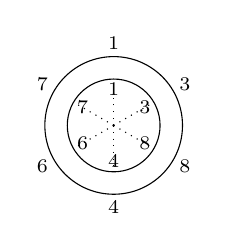
\begin{tikzpicture}[scale=0.38,baseline=-0.5ex]
\draw (0,0) circle (2.3);
\draw (0,0) circle (1.55);
\foreach \a in {30,90,150,210,270,330}{\draw[dotted] (0,0)--(\a:1.55);}
\node at (90:2.75) {\scriptsize 1};
\node at (30:2.75) {\scriptsize 3};
\node at (-30:2.75) {\scriptsize 8};
\node at (-90:2.75) {\scriptsize 4};
\node at (-150:2.75) {\scriptsize 6};
\node at (150:2.75) {\scriptsize 7};
\node at (90:1.2) {\scriptsize 1};
\node at (30:1.2) {\scriptsize 3};
\node at (-30:1.2) {\scriptsize 8};
\node at (-90:1.2) {\scriptsize 4};
\node at (-150:1.2) {\scriptsize 6};
\node at (150:1.2) {\scriptsize 7};
\end{tikzpicture}
\]
If the inner ring (or also the outer one) is turned \(60^\circ\) to the left, the new position of both rings characterizes an advancing simple cycle; with the same rotation to the right, a receding simple cycle.

To the proper substitutions belongs:

\(\alpha)\) \emph{the ordinary general interchange} of any two elements of a permutation of \(n\) elements (proper substitution in the narrower sense). Its expression is the one already mentioned. Such general interchanges are for example
\[
S_1=\begin{pmatrix}1&5&2&6&3&4\\1&2&5&6&3&4\end{pmatrix},\qquad
S_2=\begin{pmatrix}3&4&6&7&5&1&2\\3&1&6&7&5&4&2\end{pmatrix},
\]
and the same substitutions \(S_1\) and \(S_2\) can be represented by a whole series of other expressions, for example
\[
S_1=\begin{pmatrix}4&5&6&3&2&1\\4&2&6&3&5&1\end{pmatrix},\qquad
S_2=\begin{pmatrix}3&4&1&6&7&5&2\\3&1&4&6&7&5&2\end{pmatrix},
\]
as we have already noted.

\(\beta)\) \emph{The general cycle}, by which \(k\) arbitrary elements of a permutation change their places in the same way as in a simple cycle. If, for example, the permutation \((3\ 5\ 6\ 2\ 1\ 4)\) of 6 elements is given, then, in order to obtain the expression of a general cycle, we first write down a simple one, say
\[
\begin{pmatrix}2&4&1&3\\4&1&3&2\end{pmatrix}.
\]
If we then apply this substitution to the above permutation, we obtain the general cycle
\[
\begin{pmatrix}3&5&6&2&1&4\\2&5&6&4&3&1\end{pmatrix}
=
\begin{pmatrix}6&3&4&5&1&2\\6&2&1&5&3&4\end{pmatrix}
=\text{ and so on.}
\]

\emph{Remark 1.} A simple cycle as well as a simple interchange acquires the general character of proper substitutions as soon as we drop the restriction that they are to hold only for a definite permutation.

Thus by \((3\ 5)\) we shall understand a simple interchange applied, for instance, to \((4\ 2\ 3\ 5\ 1)\), whereas the general one is represented by
\[
\begin{pmatrix}4&2&3&5&1\\4&2&5&3&1\end{pmatrix}
=
\begin{pmatrix}3&4&1&5&2\\5&4&1&3&2\end{pmatrix}
=\text{ and so on.}
\]
Likewise
\[
\begin{pmatrix}6&1&4&3\\1&4&3&6\end{pmatrix}
\]
denotes the simple cycle to be applied to the permutation \((5\ 2\ 6\ 1\ 4\ 3)\), whereas the general one is characterized by
\[
\begin{pmatrix}5&2&6&1&4&3\\5&2&1&4&3&6\end{pmatrix}
=
\begin{pmatrix}1&6&4&5&2&3\\4&1&3&5&2&6\end{pmatrix}
=
\begin{pmatrix}2&1&6&5&3&4\\2&4&1&5&6&3\end{pmatrix}
=\text{ and so on.}
\]

\emph{Remark 2.} An arbitrary substitution \(S\), apart from the single one
\[
S=\begin{pmatrix}1&2&3&\cdots&n\\1&2&3&\cdots&n\end{pmatrix},
\]
which leaves everything unchanged, requires general ordinary interchanges, or also, as we shall immediately see, general cyclic interchanges.

6. \emph{Construction of the improper substitutions from one another.} The simple cycle can be constructed by simple interchanges.

Example 1. Let the simple cycle be
\[
\begin{pmatrix}2&5&3&1\\5&3&1&2\end{pmatrix}.
\]
If we let the element 2 move successively to the right, then from \((2\ 5\ 3\ 1)\) the simple interchange \((2\ 5)\) first gives \((5\ 2\ 3\ 1)\), the next simple interchange \((2\ 3)\) gives \((5\ 3\ 2\ 1)\), and finally the last \((2\ 1)\) gives the desired result \((5\ 3\ 1\ 2)\). Thus a simple cycle of 4 elements can be replaced by 3 simple interchanges.

Example 2. Let the simple cycle be
\[
\begin{pmatrix}4&6&5&8&7&3\\6&5&8&7&3&4\end{pmatrix}.
\]
Again let the first element 4 of the permutation move.
\[
\begin{array}{c@{\qquad}c}
\text{Simple interchange.} & \text{Permutation.}\\
(4\ 6)&645873\\
(4\ 5)&654873\\
(4\ 8)&658473\\
(4\ 7)&658743\\
(4\ 3)&658734
\end{array}
\]
Thus 5 simple interchanges take the place of the simple cycle of 6 elements.

One therefore easily recognizes the correctness of the theorem:
\begin{quote}
``If the difference of the position numbers of the first and last elements of a simple cycle is \(\nu\), then it can be replaced by \(\nu\) simple interchanges; \(\nu+1\) elements then take part in the cycle.''
\end{quote}

7. \emph{The general interchange can be constructed by two simple cycles.} Let there be given, 1) the general interchange
\[
S=\begin{pmatrix}2&4&1&5&3&6\\6&4&1&5&3&2\end{pmatrix}.
\]
Then the simple cycle (formed from all 6 elements)
\[
\begin{pmatrix}2&4&1&5&3&6\\4&1&5&3&6&2\end{pmatrix}
\]
first gives the permutation \((4\ 1\ 5\ 3\ 6\ 2)\).

If we apply to this the simple cycle
\[
\begin{pmatrix}4&1&5&3&6\\6&4&1&5&3\end{pmatrix},
\]
formed from five elements, then it leads to the desired result \((6\ 4\ 1\ 5\ 3\ 2)\).

Example 2. The substitution
\[
S=\begin{pmatrix}5&7&8&2&4&1&3&6\\5&4&8&2&7&1&3&6\end{pmatrix}
\]
can be split into the simple advancing cycle of four elements
\[
\begin{pmatrix}7&8&2&4\\8&2&4&7\end{pmatrix}.
\]
By it, in the permutation \((5\ 7\ 8\ 2\ 4\ 1\ 3\ 6)\), the element 7 is first brought to the place indicated by \(S\), so that one obtains \((5\ 8\ 2\ 4\ 7\ 1\ 3\ 6)\). If then one applies the receding simple cycle of three elements \(\begin{pmatrix}8&2&4\\4&8&2\end{pmatrix}\), one obtains the desired result \((5\ 4\ 8\ 2\ 7\ 1\ 3\ 6)\). The remaining examples will be understandable without further explanation.

3) General interchange:
\[
S=\begin{pmatrix}3&0&2&7&1&5&6&4\\3&0&2&5&1&7&6&4\end{pmatrix}.
\]
First cycle: \(\begin{pmatrix}7&1&5\\1&5&7\end{pmatrix}\); result: \((3\ 0\ 2\ 1\ 5\ 7\ 6\ 4)\).

Second cycle: \(\begin{pmatrix}1&5\\5&1\end{pmatrix}\); result: \((3\ 0\ 2\ 5\ 1\ 7\ 6\ 4)\).

4) General interchange:
\[
S=\begin{pmatrix}5&3&7&8&9&1&2&4&6\\5&4&7&8&9&1&2&3&6\end{pmatrix}.
\]
First cycle: \(\begin{pmatrix}3&7&8&9&1&2&4\\7&8&9&1&2&4&3\end{pmatrix}\); result: \((5\ 7\ 8\ 9\ 1\ 2\ 4\ 3\ 6)\).

Second cycle: \(\begin{pmatrix}7&8&9&1&2&4\\4&7&8&9&1&2\end{pmatrix}\); result: \((5\ 4\ 7\ 8\ 9\ 1\ 2\ 3\ 6)\).

From these four examples one can easily abstract the following law:
\begin{quote}
``If the difference of the position numbers of the two elements to be interchanged is \(\nu\), then \(\nu+1\) elements take part in the first cycle and \(\nu\) in the second. Therefore, by the preceding theorem, the first cycle consists of \(\nu\) simple interchanges, the second of \(\nu-1\). Thus, if by \emph{this} method one decomposes the general interchange into simple ones, the total sum of the latter is \(2\nu-1\), hence an odd number.''
\end{quote}
It should be noted here that this number \(2\nu-1\) depends only on the route taken above. Some systematic or even arbitrary different procedure for reducing the general interchange to simple ones will in general lead to a different number.

8. \emph{Construction of the general cycle from the general interchange.} We determine the simple cycle belonging to the general cycle, resolve it into its simple interchanges, and then form the corresponding general interchanges. These exactly replace the general cycle.

Example 1. Let the general cycle be
\[
S=\begin{pmatrix}4&3&5&1&6&2\\1&2&5&3&6&4\end{pmatrix}.
\]
The corresponding simple cycle is \(\begin{pmatrix}4&1&3&2\\1&3&2&4\end{pmatrix}\), which can itself be resolved into the simple interchanges \((4\ 1)\), \((4\ 3)\), \((4\ 2)\).

For these we form, in order, the corresponding general interchanges, and so obtain, corresponding to \((4\ 1)\),
\[
S_1=\begin{pmatrix}4&3&5&1&6&2\\1&3&5&4&6&2\end{pmatrix},
\]
then, corresponding to \((4\ 3)\),
\[
S_2=\begin{pmatrix}1&3&5&4&6&3\\1&4&5&3&6&2\end{pmatrix},
\]
and then, corresponding to \((4\ 2)\),
\[
S_3=\begin{pmatrix}1&4&5&3&6&2\\1&2&5&3&6&4\end{pmatrix},
\]
by which the desired result is reached.

Example 2. The general cycle
\[
S=\begin{pmatrix}3&5&7&9&8&2&6&4&1\\7&5&8&9&6&2&1&4&3\end{pmatrix}
\]
is to be decomposed into general interchanges. From \(S\) we determine the simple cycle
\[
\begin{pmatrix}3&7&8&6&1\\7&8&6&1&3\end{pmatrix}.
\]
It corresponds to the simple interchanges
\[
(3\ 7),\quad(3\ 8),\quad(3\ 6),\quad(3\ 1).
\]
Thus \(S\) splits into the four general interchanges
\[
S_1=\begin{pmatrix}3&5&7&9&8&2&6&4&1\\7&5&3&9&8&2&6&4&1\end{pmatrix},\quad
S_2=\begin{pmatrix}7&5&3&9&8&2&6&4&1\\7&5&8&9&3&2&6&4&1\end{pmatrix},
\]
\[
S_3=\begin{pmatrix}7&5&8&9&3&2&6&4&1\\7&5&8&9&6&2&3&4&1\end{pmatrix},\quad
S_4=\begin{pmatrix}7&5&8&9&6&2&3&4&1\\7&5&8&9&6&2&1&4&3\end{pmatrix}.
\]
From these examples one sees that the general cycle can be resolved into general interchanges in exactly the same way as the simple cycle into simple interchanges. If, therefore, \(\nu+1\) elements occur in the general cycle, it can be resolved into \(\nu\) general interchanges. (In example 1 the elements of the cycle were 4 in number, the general interchanges 3; in example 2 there were 5 elements in the cycle, hence 4 general interchanges.)

9. \emph{Construction of an arbitrary substitution by general cycles.} Let, for example, the given substitution be
\[
S=\begin{pmatrix}9&0&8&4&3&5&2&1&7&6\\1&6&5&0&9&2&8&3&4&7\end{pmatrix}.
\]
We can think of it as arising as follows: first 9 is replaced by 1, 1 by 3, and 3 again by 9; that is, the upper permutation was first subjected to the general cycle
\[
S_1=\begin{pmatrix}9&0&8&4&3&5&2&1&7&6\\1&0&8&4&9&5&2&3&7&6\end{pmatrix}.
\]
In the result of this substitution, i.e. in the lower permutation of this expression \(S_1\), the index 6 then took the place of 0, the index 7 the place of 6, the index 4 the place of 7, and finally the index zero again the place of 4; that is, it was subjected to a change effected by the general cycle
\[
S_2=\begin{pmatrix}1&0&8&4&9&5&2&3&7&6\\1&6&8&0&9&5&2&3&4&7\end{pmatrix}.
\]
From the lower permutation of the substitution \(S_2\) one finally reaches the desired lower permutation in the expression \(S\) by replacing 8 by 5, 5 by 2, and 2 again by 8, hence by applying to it the general cycle
\[
S_3=\begin{pmatrix}1&6&8&0&9&5&2&3&4&7\\1&6&5&0&9&2&8&3&4&7\end{pmatrix}.
\]
Thus we see that the general substitution \(S\) can be replaced by the three general cycles \(S_1,S_2,S_3\).

The number of cycles that can occur for a general substitution cannot be given in advance; but it is rapidly found if, starting for instance with the first digit on the left, one proceeds by the method indicated three times in the preceding example. Every time we return in this way to the initial digit, the first cycle is closed, and the determination of the second cycle can then begin with the next index which has not already occurred in the first.

It may of course happen that only one cycle occurs at all, i.e. that the general substitution itself represents a single cycle, as in the example
\[
(2)\qquad S=\begin{pmatrix}5&9&8&2&3&4&1&7&6\\9&2&5&1&4&6&3&8&7\end{pmatrix},
\]
or also that \(S\) contains cycles with a single element, as for instance the substitution
\[
(3)\qquad S=\begin{pmatrix}5&1&8&2&3&4&7&6\\2&1&5&4&3&6&8&7\end{pmatrix}.
\]
It splits into the cycle
\[
\begin{pmatrix}5&2&4&6&7&8\\2&4&6&7&8&5\end{pmatrix}
\]
with six elements and into the two one-termed cycles \((1),(3)\).

If by the stated method one has determined the number \(\nu\) of cycles which can represent a general substitution, one obtains the number of general interchanges as follows. Let the number of elements of the first cycle be \(\alpha_1\), that of the second \(\alpha_2\), and so on, that of the \(\nu^{\mathrm{th}}\) be \(\alpha_\nu\). Since all elements must be exhausted by all cycles,
\[
\sum\alpha_\varrho=\alpha_1+\alpha_2+\cdots+\alpha_\nu=n.
\]
But by no. 8 the general cycle of \(\alpha_\varrho\) elements consists of \(\alpha_\varrho-1\) interchanges; hence the sum of all general interchanges which can replace the general substitution is
\[
\sum\alpha_\varrho-(1+1+\cdots\,\nu\text{ times})=n-\nu.
\]
It may be mentioned once again that this number depends only on the method used here to determine it.

10. \emph{Determining the principal class (see no. 4) to which a substitution belongs.} This problem could best be settled directly on the product of differences by making in it the individual interchanges one after another. But perhaps it can be solved more easily by taking account of individual features of the substitutions that we have now discussed. We see the following.

\(\alpha)\) Since the simple interchange refers to a single definite, though arbitrarily given, permutation, for simplicity we may assume this arbitrarily given one to be the \emph{well-ordered} permutation. This being assumed, a simple interchange of two neighboring indices \(\alpha_\varrho\) and \(\alpha_{\varrho+1}\), which can of course then differ only by 1, when applied to the product of differences of the indices, can change only the sign of the single difference \((\alpha_\varrho-\alpha_{\varrho+1})\), since in all other differences the distance of the index from \(\alpha_\varrho\) or \(\alpha_{\varrho+1}\) is at least two units, so that changing the minuend or subtrahend by 1 cannot cause a change of sign. Thus with this single factor \((\alpha_\varrho-\alpha_{\varrho+1})\) the entire product changes its sign, i.e. ``the simple interchange belongs to the second principal class.'' But this also gives the classification of the remaining substitutions.

\(\beta)\) The simple cycle of \(\nu+1\) elements belongs, by (6), to the first or second principal class according as \(\nu\) (= the number of its simple interchanges) is even or odd.

\(\gamma)\) The general interchange always belongs to the second principal class, since by no. 7 it consists of \(2\nu-1\), hence of an odd number of simple interchanges.

\(\delta)\) The general cycle behaves like the simple one, since the general interchanges by which the former can be replaced belong, like simple interchanges, to the second principal class.

\(\varepsilon)\) Finally, the arbitrary substitution consists of \(n-\nu\) general interchanges, where \(n\) is the number of elements and \(\nu\) is the number of general cycles replacing the substitution. According as this difference is even or odd, the substitution belongs to the first or second principal class.

11. We apply these features to the examples already treated.

\(\alpha)\) In the permutation \((5\ 3\ 4\ 2\ 1)\) the simple interchange \((2\ 1)\) changes the sign of the product of differences
\[
\begin{gathered}
(1-2)(1-3)(1-4)(1-5)=P\\
(2-3)(2-4)(2-5)\\
(3-4)(3-5)\\
(4-5)
\end{gathered}
\]
for in it only the first factor changes its sign, the remaining ones pass into one another; one obtains
\[
\begin{gathered}
(2-1)(2-3)(2-4)(2-5)=-P.\\
(1-3)(1-4)(1-5)\\
(3-4)(3-5)\\
(4-5).
\end{gathered}
\]

\(\beta)\) The first simple cycle in no. 6,
\[
\begin{pmatrix}2&5&3&1\\5&3&1&2\end{pmatrix}
\]
was composed of three simple interchanges \((2\ 5),(2\ 3),(2\ 1)\), and therefore belongs to the second class, whereas, for example, the simple cycle
\[
\begin{pmatrix}2&5&3&1&4\\5&3&1&4&2\end{pmatrix},
\]
because it consists of the four simple interchanges \((2\ 5),(2\ 3),(2\ 1),(2\ 4)\), is to be counted in the first principal class.

\(\gamma)\) The general interchange
\[
S=\begin{pmatrix}2&4&1&5&3&6\\6&4&1&5&3&2\end{pmatrix}\quad \text{no. 7, example 1,}
\]
was replaced by the two simple cycles
\[
S_1=\begin{pmatrix}2&4&1&5&3&6\\4&1&5&3&6&2\end{pmatrix}
\quad\text{and}\quad
S_2=\begin{pmatrix}4&1&5&3&6\\6&4&1&5&3\end{pmatrix}.
\]
The first consists of five, the second of four simple interchanges. Since their sum is \(9\), \(S\) belongs to the second class of substitutions; the assertion is easily verified directly on the product of differences.

\(\delta)\) The substitution no. 7, example 2,
\[
S=\begin{pmatrix}5&7&8&2&4&1&3&6\\5&4&8&2&7&1&3&6\end{pmatrix}
\]
split into the cycles
\[
S_1=\begin{pmatrix}7&8&2&4\\8&2&4&7\end{pmatrix},\qquad
S_2=\begin{pmatrix}8&2&4\\4&8&2\end{pmatrix},
\]
the first of which consists of the three simple interchanges \((7\ 8),(7\ 2),(7\ 4)\), the second of the two interchanges \((8\ 2),(8\ 4)\). Their sum is \(5\), again an odd number.

\(\varepsilon)\) The general cycle
\[
S=\begin{pmatrix}4&3&5&1&6&2\\1&2&5&3&6&4\end{pmatrix}
\]
in no. 8 was decomposed into the three general interchanges
\[
S_1=\begin{pmatrix}4&3&5&1&6&2\\1&3&5&4&6&2\end{pmatrix},\quad
S_2=\begin{pmatrix}1&3&5&4&6&2\\1&4&5&3&6&2\end{pmatrix},\quad
S_3=\begin{pmatrix}1&4&5&3&6&2\\1&2&5&3&6&4\end{pmatrix}.
\]
For \(S_1\), the difference of the position numbers to be interchanged is \(\nu_1=3\), hence the corresponding number of simple interchanges is \(2\nu_1-1=5\). Further, for \(S_2\), \(\nu_2=2\), so the number of simple interchanges is \(2\nu_2-1=3\); finally, for \(S_3\), \(\nu_3=4\), so the number of simple interchanges is \(2\nu_3-1=7\). The sum of all interchanges is therefore \(5+3+7=15\).

Hence \(S\) belongs to the second principal class. If we analyze in the same way the second example given in the same section, we find
\[
2\nu_1-1=3,\quad 2\nu_2-1=3,\quad 2\nu_3-1=3,\quad 2\nu_4-1=3.
\]
The sum of these four odd numbers gives an even number, i.e. this substitution belongs to the first principal class.

\(\zeta)\) Finally consider the arbitrary substitution
\[
S=\begin{pmatrix}9&0&8&4&3&5&2&1&7&6\\1&6&5&0&9&2&8&3&4&7\end{pmatrix}
\]
in no. 9. We decomposed it into the three general cycles
\[
S_1=\begin{pmatrix}9&0&8&4&3&5&2&1&7&6\\1&0&8&4&9&5&2&3&7&6\end{pmatrix},
\quad
S_2=\begin{pmatrix}1&0&8&4&9&5&2&3&7&6\\1&6&8&0&8&5&2&3&4&7\end{pmatrix},
\]
\[
S_3=\begin{pmatrix}1&6&8&0&9&5&2&3&4&7\\1&6&5&0&9&2&8&3&4&7\end{pmatrix},
\]
whose simple cycles are
\[
\begin{pmatrix}9&3&1\\1&9&3\end{pmatrix},\qquad
\begin{pmatrix}0&4&7&6\\6&0&4&7\end{pmatrix},\qquad
\begin{pmatrix}8&5&2\\5&2&8\end{pmatrix}.
\]
Thus to the first cycle belong two, to the second three, and to the third again two general interchanges. Their number is consequently \(7\), and since every general interchange can be resolved only into an odd number of simple ones, the class of this substitution is the second.

\(\eta)\) On the other hand, the substitution
\[
S=\begin{pmatrix}5&6&7&3&4&2\\3&4&6&2&7&5\end{pmatrix},
\]
which splits into two general cycles, to which the simple cycles
\[
\begin{pmatrix}5&3&2\\3&2&5\end{pmatrix}
\quad\text{and}\quad
\begin{pmatrix}6&4&7\\4&7&6\end{pmatrix}
\]
correspond, belongs to the first principal class, because in the two general cycles three elements occur in each, so that together they can be replaced by \(2+2=4\), i.e. by an even number of general interchanges.

12. \emph{Classification of a substitution by counting derangements.} A further means for determining the class of a substitution \(S\) is supplied by counting the derangements in the two permutations of \(S\). Namely the following theorem holds:
\begin{quote}
``If a substitution belongs to the first class, the difference of the derangements in the upper and lower permutation is even; if it belongs to the second class, it is odd.''
\end{quote}
\end{document}
